\documentclass[12pt,a4paper]{article}

% Packages
\usepackage{graphicx} % For including images
\usepackage{fancyhdr} % For customizing headers and footers
\usepackage{amsmath} % For mathematical symbols and equations
\usepackage{cite} % For citing references
\usepackage{setspace} % For setting spacing between lines
\usepackage[margin=1in]{geometry} % For setting page margins
\usepackage{hyperref} % For creating hyperlinks
\usepackage{multicol} % For multi-column layout
\usepackage{booktabs} % for better looking tables
\usepackage{multirow} % for combining rows

\usepackage{tikz} % for scatterplot graph
\usepackage{pgfplots} % for scatterplot graph
\pgfplotsset{compat=1.16} % for scatterplot graph
\usepgfplotslibrary{statistics} % for scatterplot graph
\usepackage{pgfplotstable} 

\usepackage{pgf,tikz,pgfplots}
\pgfplotsset{compat=1.15}
\usepackage{mathrsfs}
\usetikzlibrary{arrows}

\usepackage{physics}
\usepackage{amsmath}
\usepackage{tikz}
\usepackage{mathdots}
\usepackage{yhmath}
\usepackage{cancel}
\usepackage{color}
\usepackage{siunitx}
\usepackage{array}
\usepackage{multirow}
\usepackage{amssymb}
\usepackage{gensymb}
\usepackage{tabularx}
\usepackage{extarrows}
\usepackage{booktabs}
\usetikzlibrary{fadings}
\usetikzlibrary{patterns}
\usetikzlibrary{shadows.blur}
\usetikzlibrary{shapes}


% Page style
\pagestyle{fancy}
\fancyhf{} % Clear all headers and footers
\renewcommand{\headrulewidth}{0pt} % Remove header line
\fancyfoot[C]{\thepage} % Page number in center of footer

% Title page
\title{\textbf{DP Physics Internal Assessment} \\ \vspace{0.5cm} \large{Name: [Insert Your Name]} \\ \vspace{0.5cm} \large{Candidate Number: [Insert Candidate Number]} \\ \vspace{0.5cm} \large{Word Count: [Insert Word Count]}}
\author{}
\date{February 17, 2023}
\setlength{\parindent}{0pt} % Disable paragraph indentation

\begin{document}

% Title page
\maketitle

% Abstract
\section*{Abstract}
[Insert your abstract here. The abstract should be a brief summary of your investigation and should not exceed 300 words.]

% Table of contents
\newpage
\tableofcontents
\newpage

% Introduction
\section{Introduction}
[Insert your introduction here. This should include a brief background of your investigation and your research question.]


\begin{figure}
\centering
\tikzset{every picture/.style={line width=0.75pt}} %set default line width to 0.75pt        

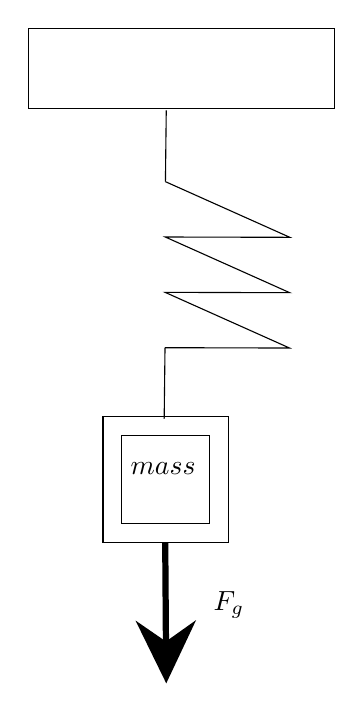
\begin{tikzpicture}[x=0.75pt,y=0.75pt,yscale=-1,xscale=1]
%uncomment if require: \path (0,353); %set diagram left start at 0, and has height of 353

%Shape: Rectangle [id:dp22882877139676516] 
\draw   (123,35) -- (270.5,35) -- (270.5,73.63) -- (123,73.63) -- cycle ;
%Shape: Sawtooth Wave Form [id:dp19337295131046361] 
\draw   (189.1,108.92) -- (249.03,135.74) -- (189.04,135.59) -- (248.96,162.41) -- (188.97,162.26) -- (248.9,189.08) -- (188.9,188.92) ;
%Straight Lines [id:da1849549639195066] 
\draw    (189.5,74.63) -- (189.1,108.92) ;
%Straight Lines [id:da4755139715547929] 
\draw    (188.9,188.92) -- (188.5,223.21) ;
%Shape: Frame [id:dp027554970721731742] 
\draw   (159,222) -- (219.5,222) -- (219.5,282.63) -- (159,282.63) -- cycle(210.43,231.08) -- (168.08,231.08) -- (168.08,273.56) -- (210.43,273.56) -- cycle ;
%Straight Lines [id:da74941850577794] 
\draw [line width=2.25]    (189,283) -- (189.46,345.63) ;
\draw [shift={(189.5,350.63)}, rotate = 269.58] [fill={rgb, 255:red, 0; green, 0; blue, 0 }  ][line width=0.08]  [draw opacity=0] (30.36,-14.59) -- (0,0) -- (30.36,14.59) -- (20.16,0) -- cycle    ;

% Text Node
\draw (171.08,243.08) node [anchor=north west][inner sep=0.75pt]   [align=left] {$\displaystyle mass$};
% Text Node
\draw (211,305) node [anchor=north west][inner sep=0.75pt]   [align=left] {$\displaystyle F_{g}$};
\end{tikzpicture}
\caption{TikZ Figure Exported from Mathcha.io}
\label{fig:mathcha}
\end{figure}

% Methodology
\section{Methodology}
[Insert your methodology here. This should include a description of the equipment and materials used, the procedure followed, and the data collected.]

\begin{table}[ht]
\centering
\label{tab:rawdata}
\begin{tabular}{@{}cccccc@{}}
\toprule
\multirow{2}{*}{\textbf{Change in IV}} & \multicolumn{5}{c}{\textbf{Trials}} \\
\cmidrule(l){2-6}
& \textbf{1} & \textbf{2} & \textbf{3} & \textbf{Average} & \textbf{SD} \\
\midrule
1 & 3.5 & 3.6 & 3.7 & 3.6 & 0.1 \\
2 & 4.2 & 4.3 & 4.4 & 4.3 & 0.1 \\
3 & 5.1 & 5.2 & 5.3 & 5.2 & 0.1 \\
4 & 6.0 & 6.1 & 6.2 & 6.1 & 0.1 \\
5 & 7.2 & 7.3 & 7.4 & 7.3 & 0.1 \\
\bottomrule
\end{tabular}
\caption{Raw Data Table}
\end{table}

% Analysis
\section{Analysis}
[Insert your data analysis here. This should include graphs, tables, and calculations, as well as a discussion of your results.]
\\
\\
\begin{center}
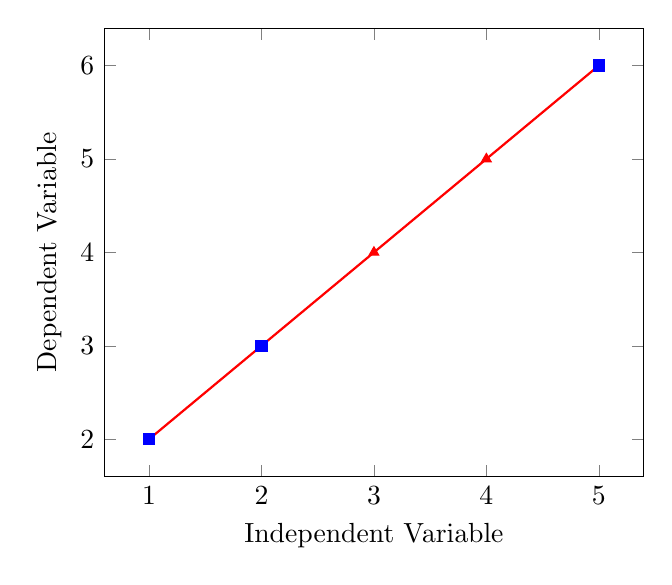
\begin{tikzpicture}
\begin{axis}[    xlabel=Independent Variable,    ylabel=Dependent Variable,    scatter/classes={        a={mark=square*,blue},        b={mark=triangle*,red}    }]

\addplot[scatter,only marks,scatter src=explicit symbolic]
table[x=x,y=y,meta=label,col sep=comma] {
x,y,label
1,2,a
2,3,a
3,4,b
4,5,b
5,6,a
};

\addplot [no markers, thick, red]
table [x=x, y={create col/linear regression={y=y}}] {
x y
1 2
2 3
3 4
4 5
5 6
};

\end{axis}
\end{tikzpicture}
\end{center}

\begin{figure}
\centering
\definecolor{zzttqq}{rgb}{0.6,0.2,0}
\definecolor{xdxdff}{rgb}{0.49019607843137253,0.49019607843137253,1}
\definecolor{ududff}{rgb}{0.30196078431372547,0.30196078431372547,1}
\begin{tikzpicture}[line cap=round,line join=round,>=triangle 45,x=1cm,y=1cm]
\clip(-10.24,-6.87) rectangle (10.24,6.87);
\fill[line width=2pt,color=zzttqq,fill=zzttqq,fill opacity=0.10000000149011612] (-2.78,0.21) -- (-1.3,2.79) -- (0.0738131434144167,-0.6281828812825558) -- cycle;
\draw [line width=2pt] (-2.78,0.21) circle (2.9743570733857765cm);
\draw [line width=2pt,color=zzttqq] (-2.78,0.21)-- (-1.3,2.79);
\draw [line width=2pt,color=zzttqq] (-1.3,2.79)-- (0.0738131434144167,-0.6281828812825558);
\draw [line width=2pt,color=zzttqq] (0.0738131434144167,-0.6281828812825558)-- (-2.78,0.21);
\begin{scriptsize}
\draw [fill=ududff] (-2.78,0.21) circle (2.5pt);
\draw[color=ududff] (-2.7,0.64) node {$A$};
\draw [fill=ududff] (-1.3,2.79) circle (2.5pt);
\draw[color=ududff] (-1.14,3.22) node {$B$};
\draw [fill=xdxdff] (0.0738131434144167,-0.6281828812825558) circle (2.5pt);
\draw[color=xdxdff] (0.5,-0.2) node {$C$};
\end{scriptsize}
\end{tikzpicture}
\caption{TikZ Figure Exported from Geogebra}
\label{fig:my_label}
\end{figure}


% Conclusion
\section{Conclusion}
[Insert your conclusion here. This should include a summary of your investigation and your findings, as well as a discussion of any limitations and suggestions for further research.]

% References
\section*{References}
[Insert your references here. Make sure to use the appropriate citation style for your subject area.]

% Appendices
\newpage
\section*{Appendices}
[Insert any appendices here. This could include raw data, calculations, or additional graphs and tables.]

\end{document}